\chapter{Simulations}\label{c:simulations}

This chapter details the attempts at reproducing micropillar tensile tests on single crystal Ni, performed by Alan Xu and Dhriti Bhattacharyya at ANSTO Sydney.

\section{Methodology}

\subsection{Experimental setup}

In total, eight loading tests were carried out.
\begin{enumerate}
    \item Loading in the $\langle 1\, 0\, 0 \rangle$:
          \begin{enumerate}
              \item Two tests with a loading rate of $\SI{5}{\nano\metre\per\second}$
              \item Two tests with a loading rate of $\SI{500}{\nano\metre\per\second}$.
          \end{enumerate}
    \item Loading in the $\langle 1\, 1\, 0 \rangle$:
          \begin{enumerate}
              \item Two tests with a loading rate of $\SI{5}{\nano\metre\per\second}$
              \item Two tests with a loading rate of $\SI{500}{\nano\metre\per\second}$.
          \end{enumerate}
\end{enumerate}

The cross-section of the micropillars was well-known at $\SI{12}{\micro\metre} \times \SI{12}{\micro\metre}$, however the length was postulated to be $\sim \SI{30}{\micro\metre}$.

The initial dislocation configuration was not well known but was postulated to be approximately 10 dislocations per square micron. The total length of mobile dislocations influences how much plasticity we observe. Furthermore, the Frank-Reed (FR) source length was unknown. A dislocation line's yield stress is inversely proportional to its length,
\begin{align}
    \sigma_\rvar{y} & = \dfrac{\mu b}{l}\,,
\end{align}
where $\sigma_\rvar{y}$ is the yield stress, $\mu$ the shear modulus, $b = \lVert \vec{b} \rVert$, and $l$ the dislocation line length. Both of these parameters had to be estimated and refined by running probing simulations.

The tensile tests were set up as shown in \cref{f:expSetup}. The pillars were placed under tensile load in the $x$-direction but were free to move in the $xy$-plane, which would naturally happen as dislocations exit the surface and create slip steps.
\begin{figure}
    \centering
    \begin{subfigure}[t]{0.45\linewidth}
        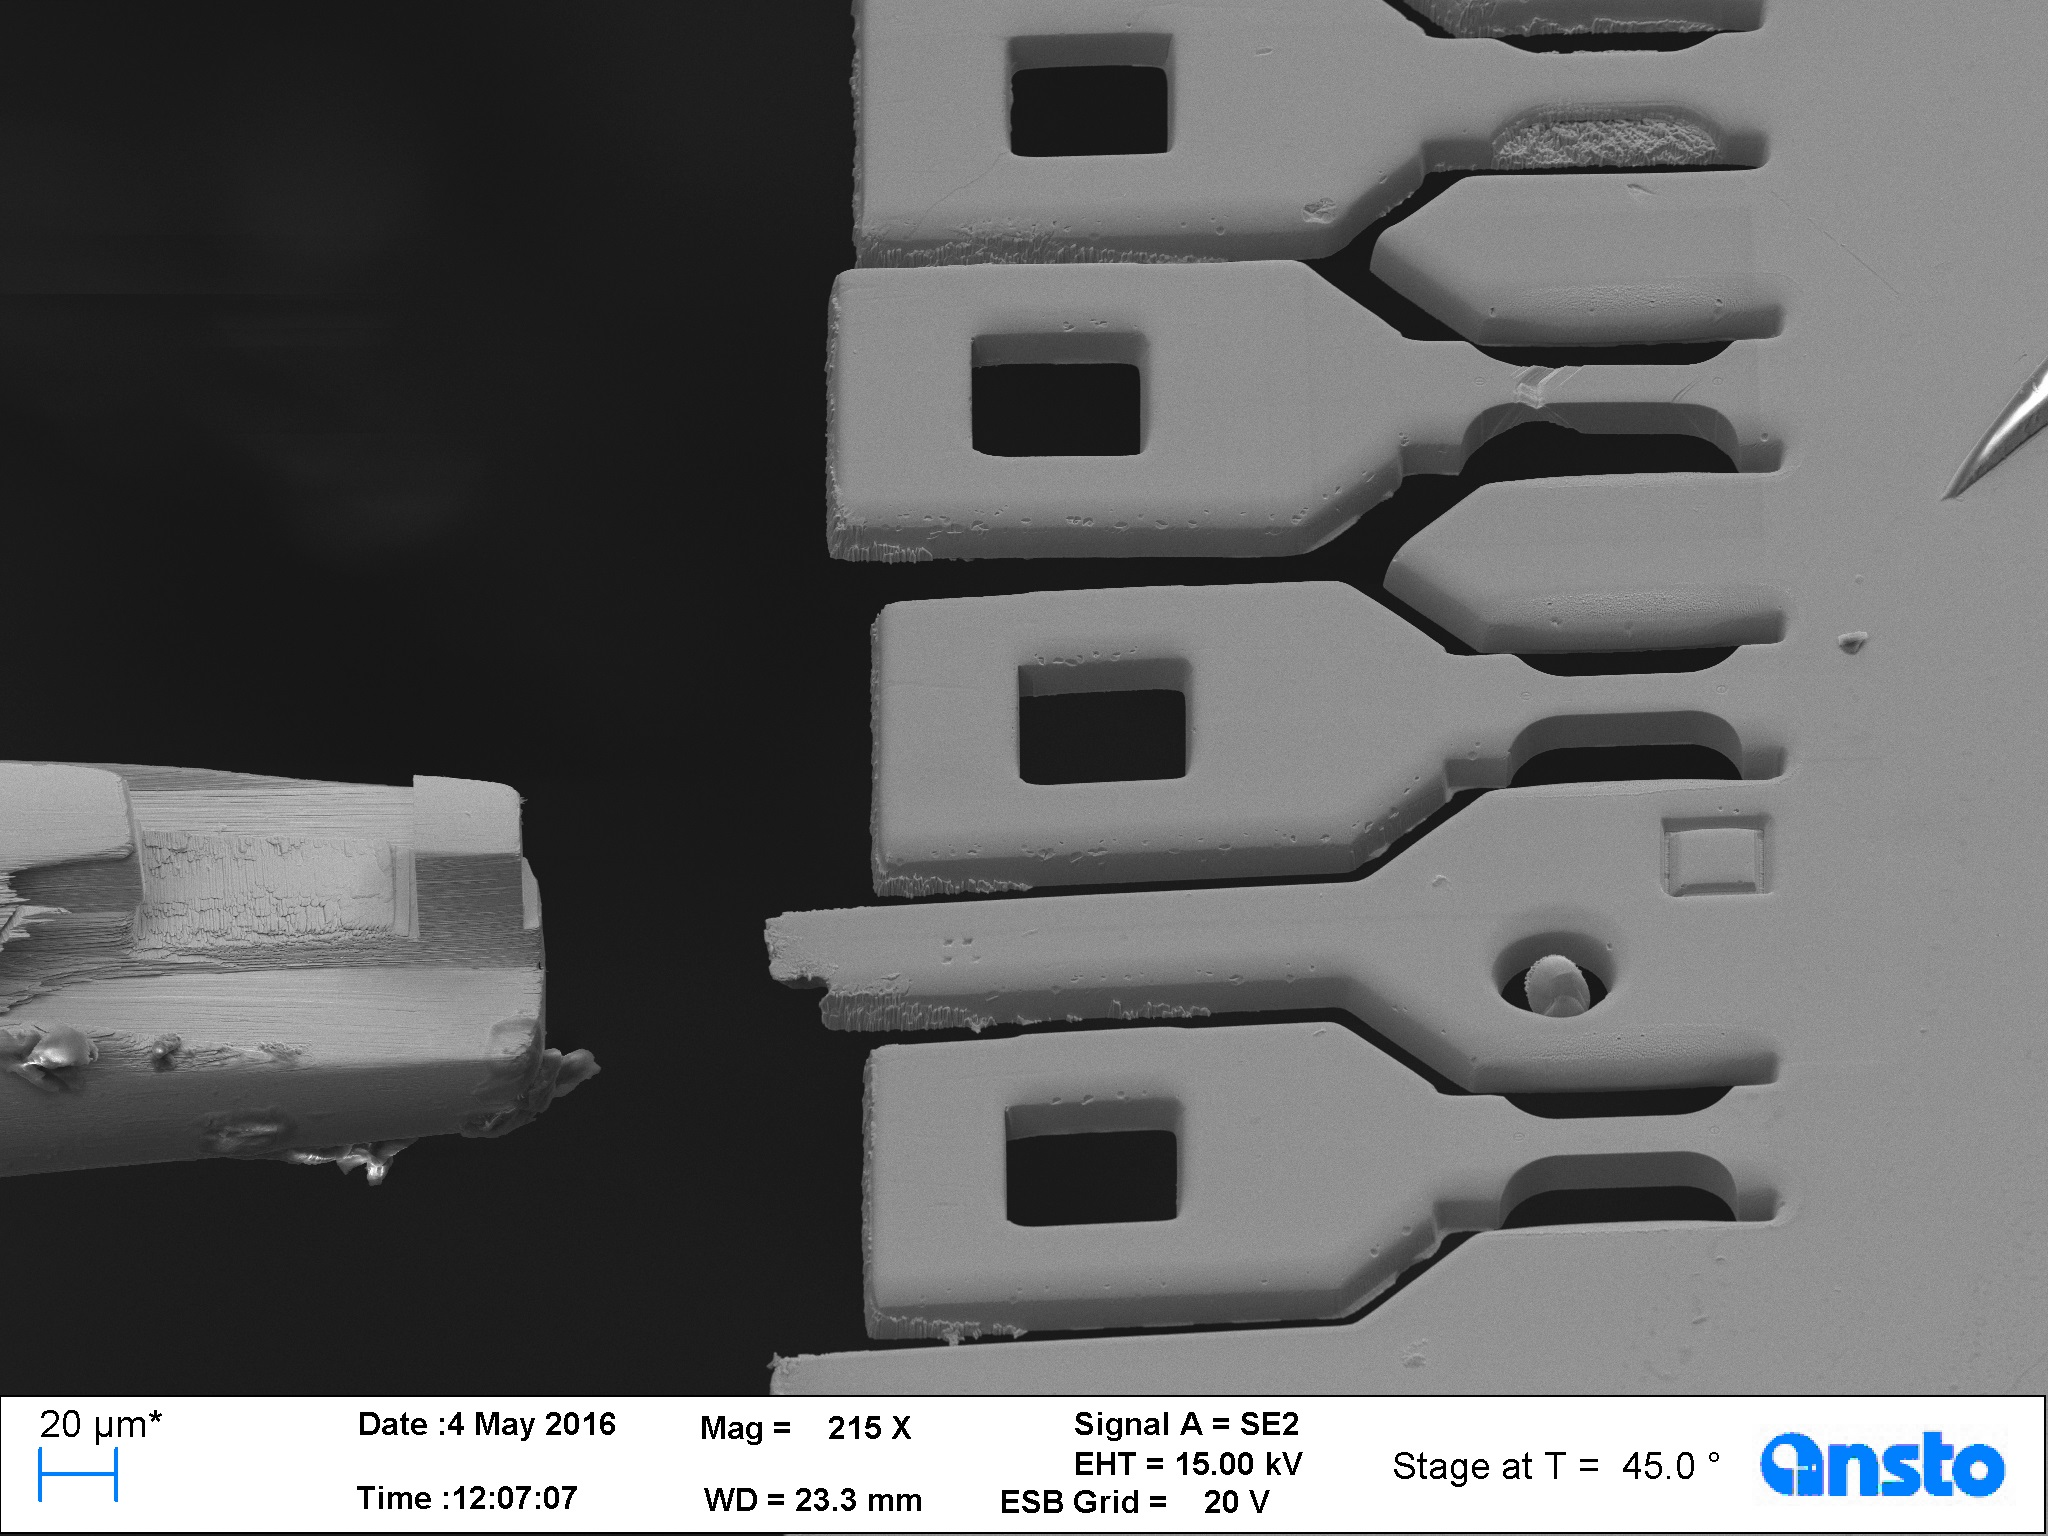
\includegraphics[width=\linewidth]{../data/Ni024.jpg}
        \caption[Stage for micropillar tensile tests.]{Stage for micropillar tensile tests. Ensemble setup, pillars are pulled from the square hole. They are allowed to freely move in the $yz$-plane.}
    \end{subfigure}
    ~
    \begin{subfigure}[t]{0.45\linewidth}
        \centering
        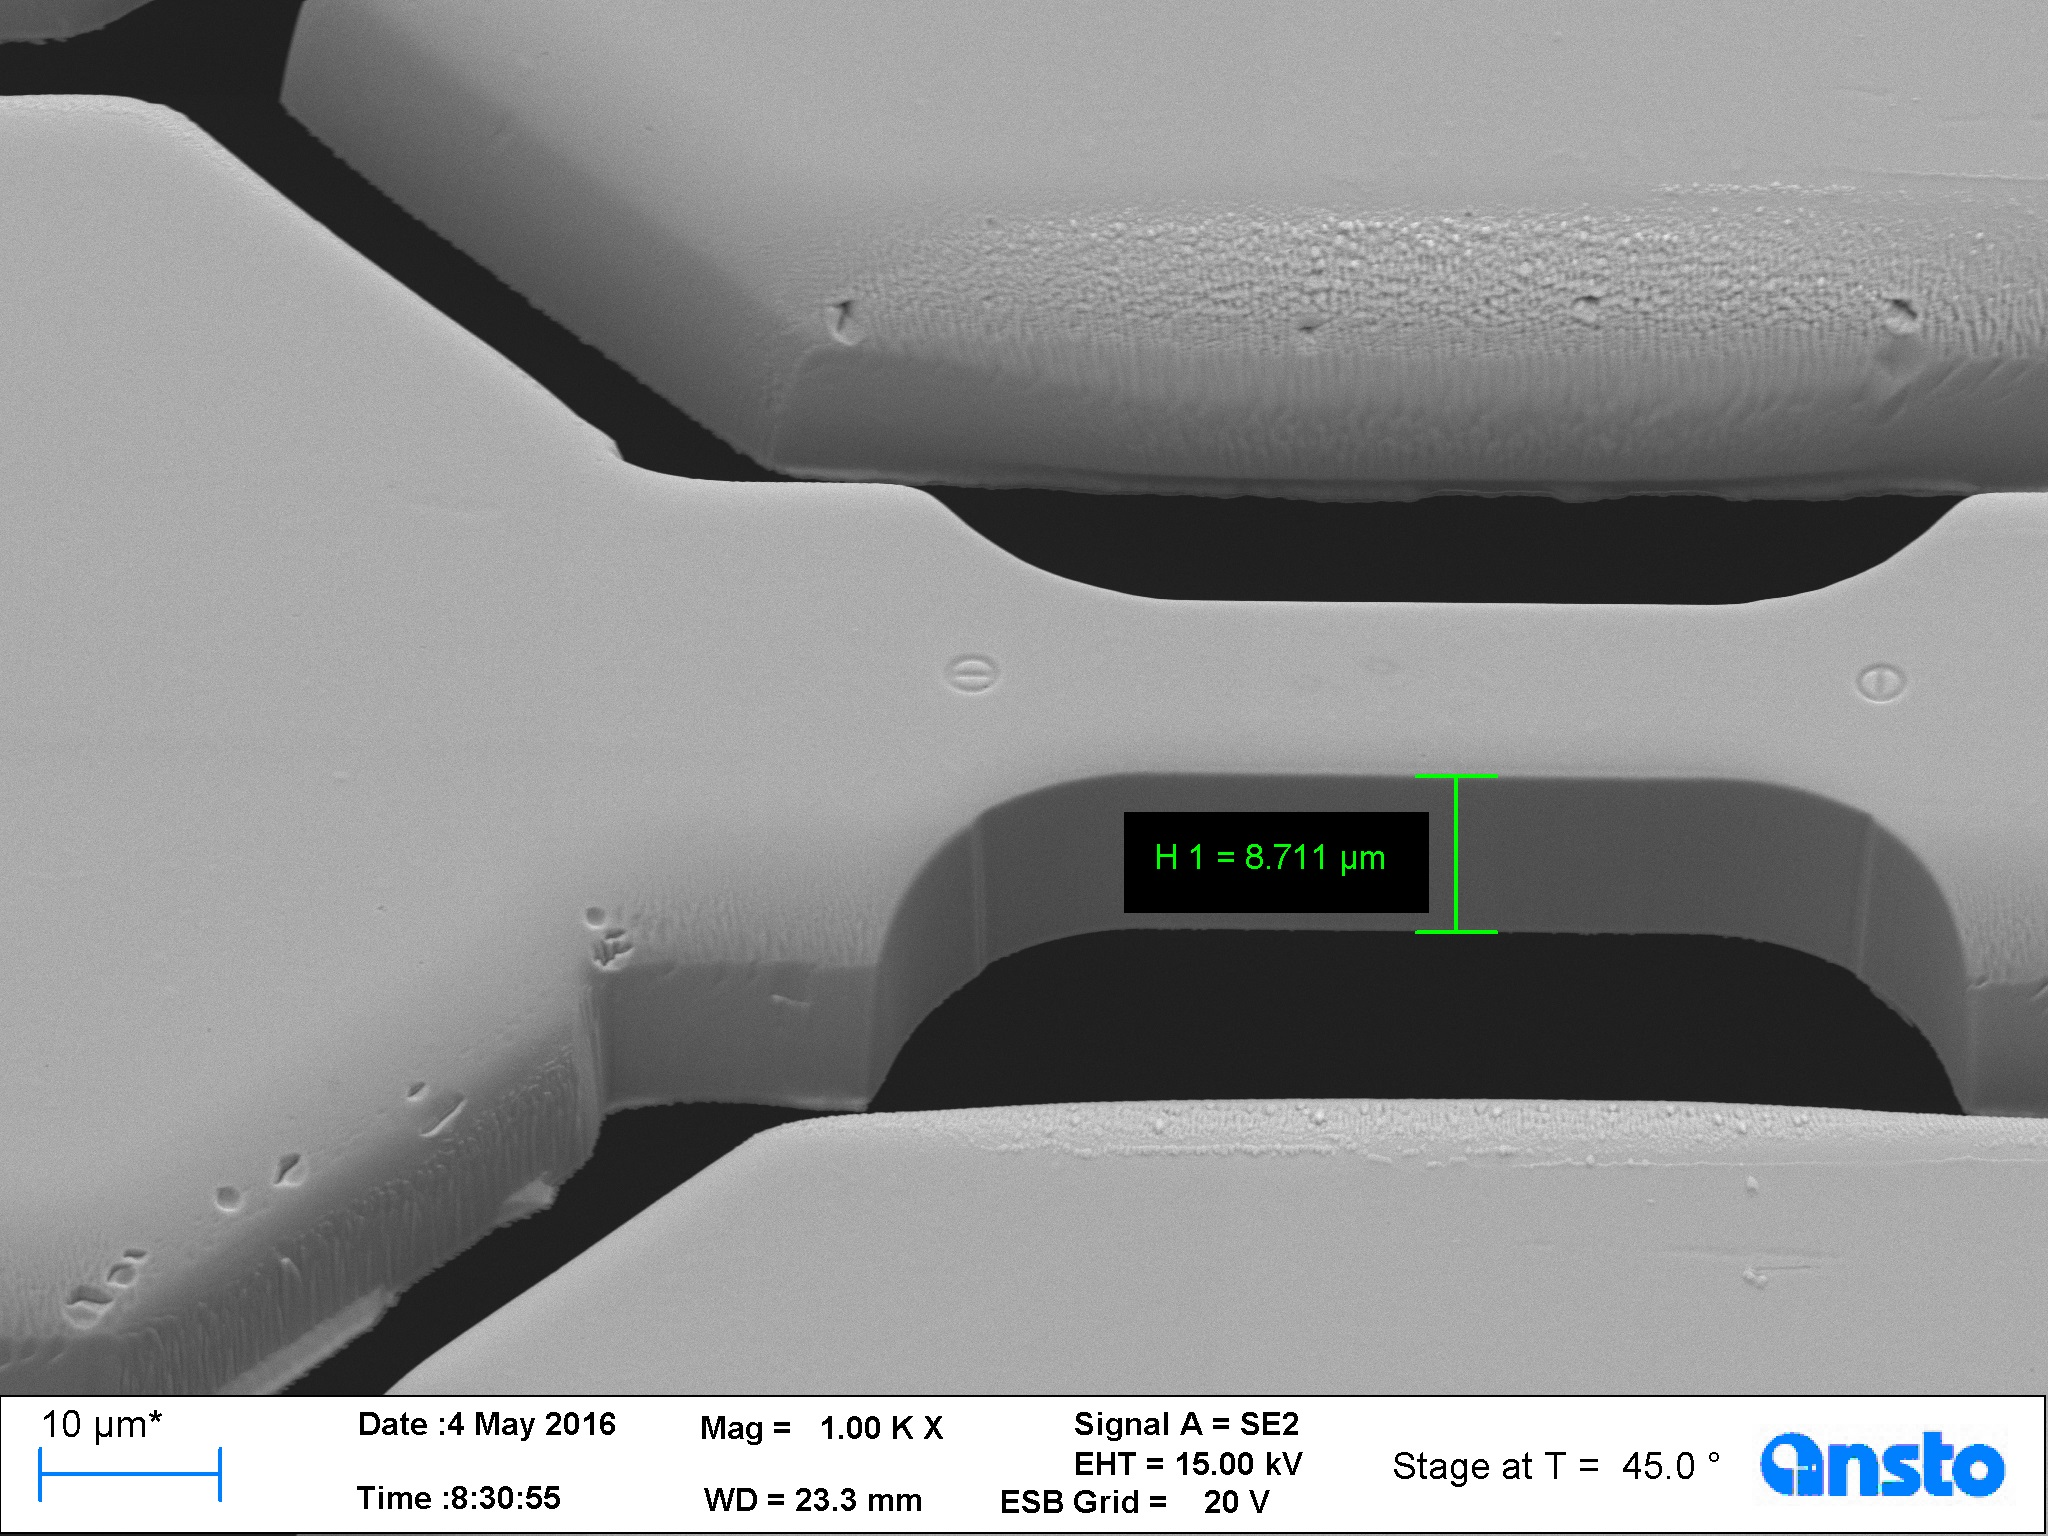
\includegraphics[width=\linewidth]{../data/Ni000.jpg}
        \caption[Close up of the initial state of a single pillar.]{Close up of the initial state of a single pillar. Camera is at $\SI{45}{\degree}$, square cross-section measures $\SI{12}{\micro\metre}$ per side, length is $\sim \SI{30}{\micro\metre}$.}
    \end{subfigure}
    \caption{Experimental stage for tensile tests on Ni micropillars.}
    \label{f:expSetup}
\end{figure}
The load was applied until the pillars failed by necking, as shown in \cref{f:necking}.
\begin{figure}
    \centering
    \begin{subfigure}[t]{0.3\linewidth}
        \centering
        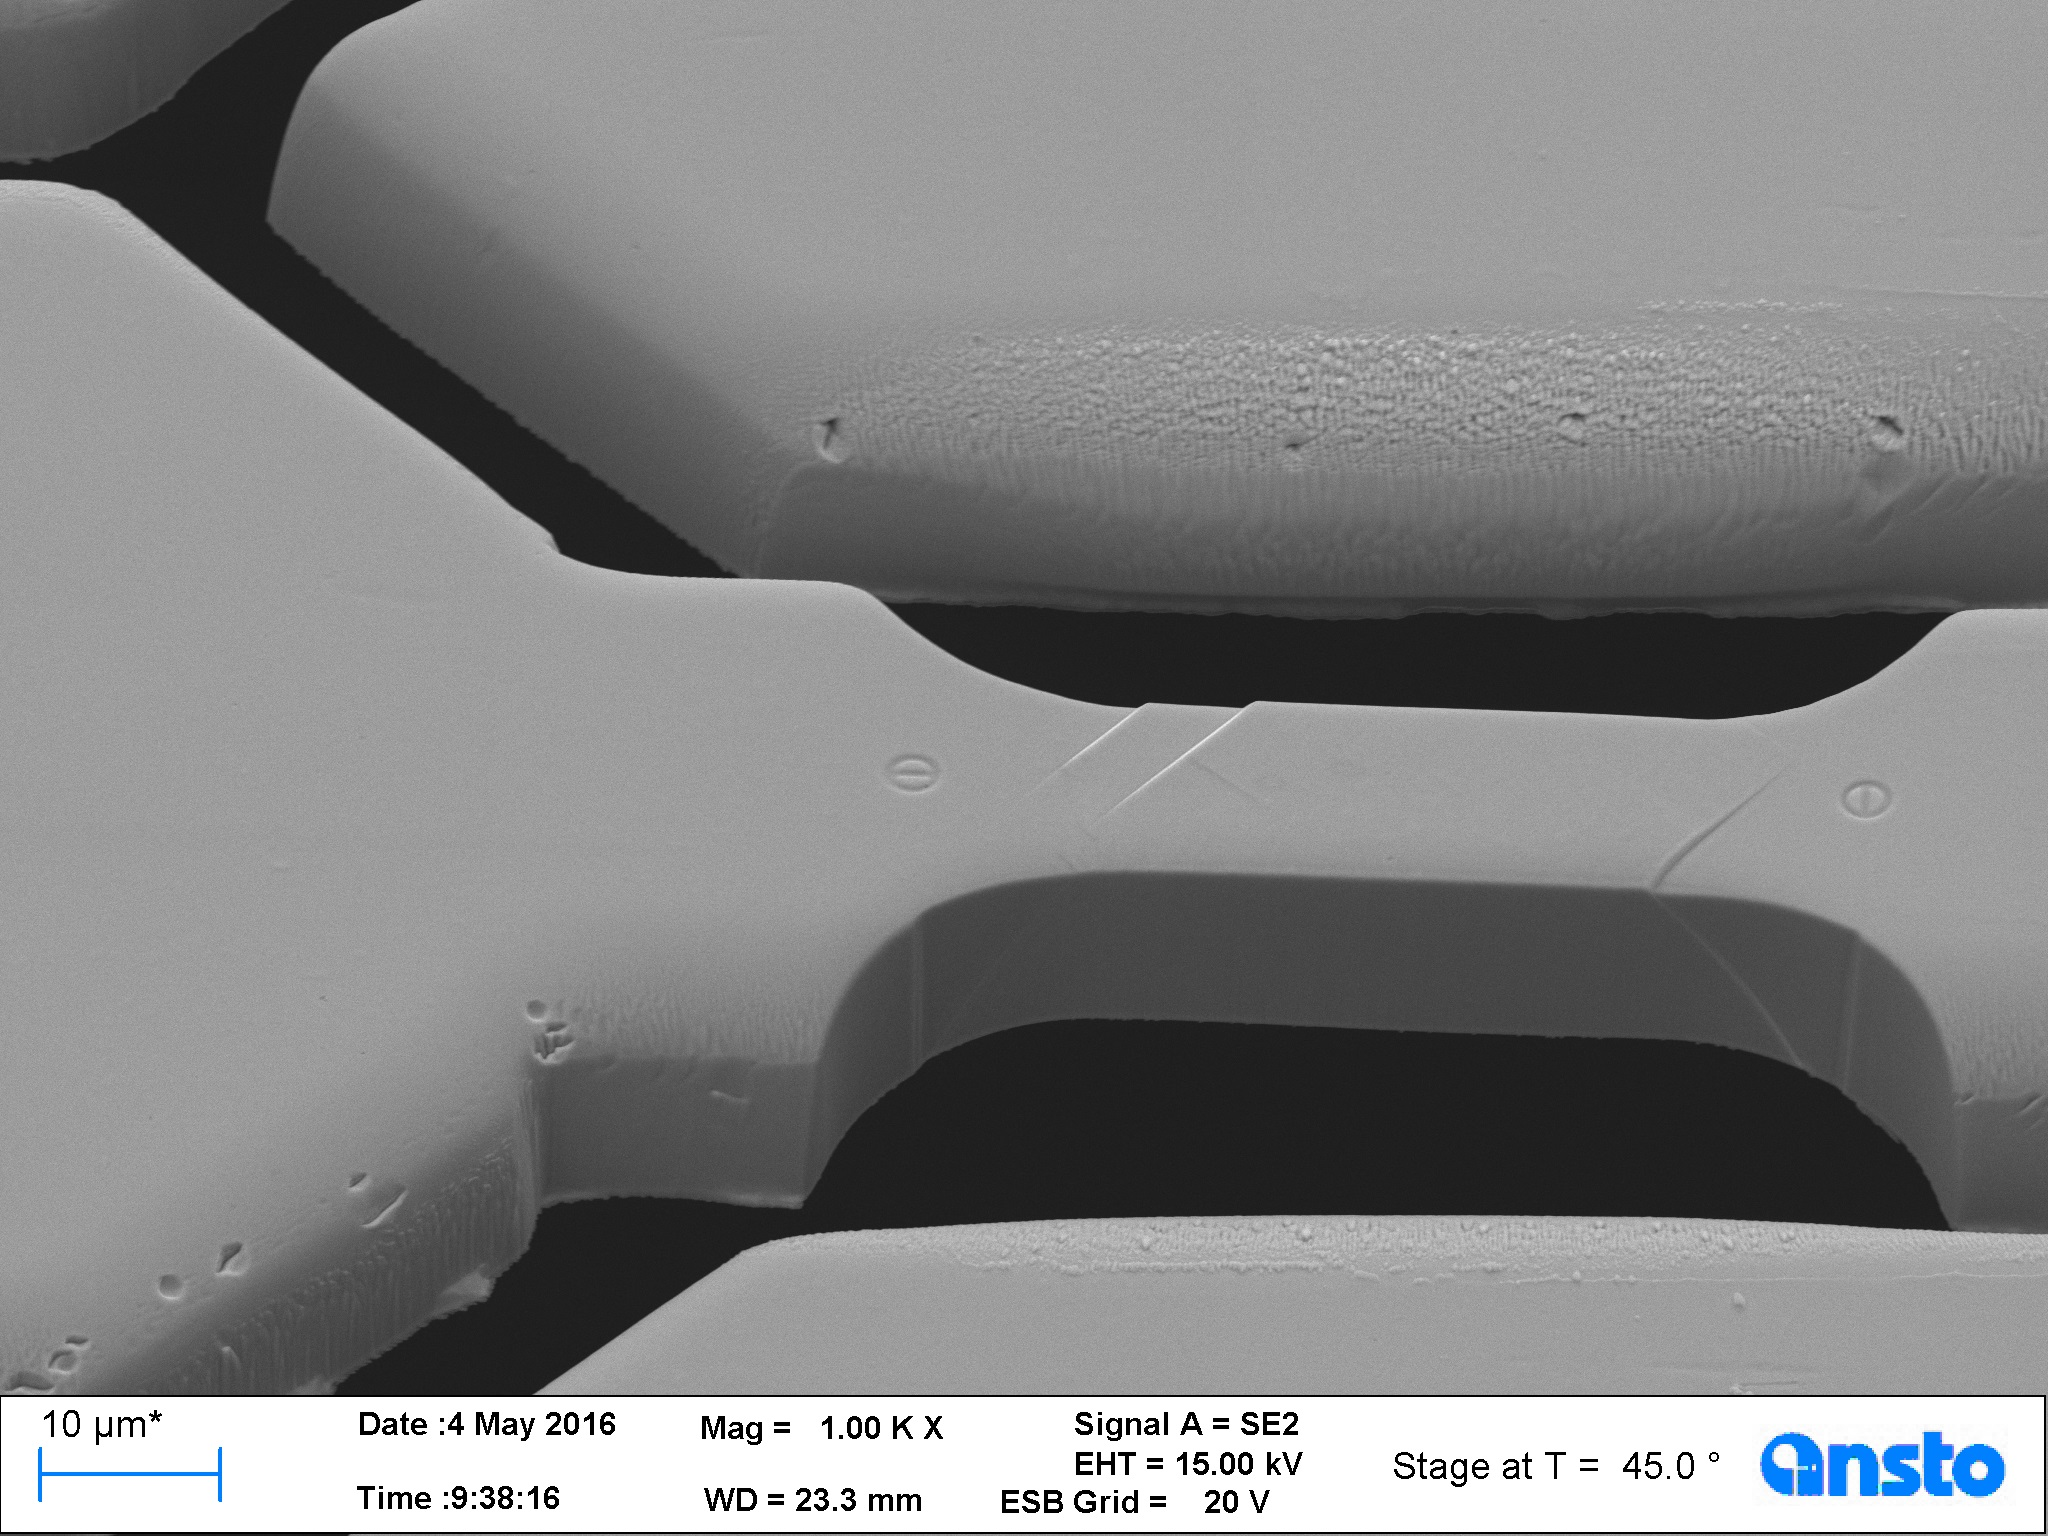
\includegraphics[width=\linewidth]{../data/Ni016.jpg}
    \end{subfigure}
    ~
    \begin{subfigure}[t]{0.3\linewidth}
        \centering
        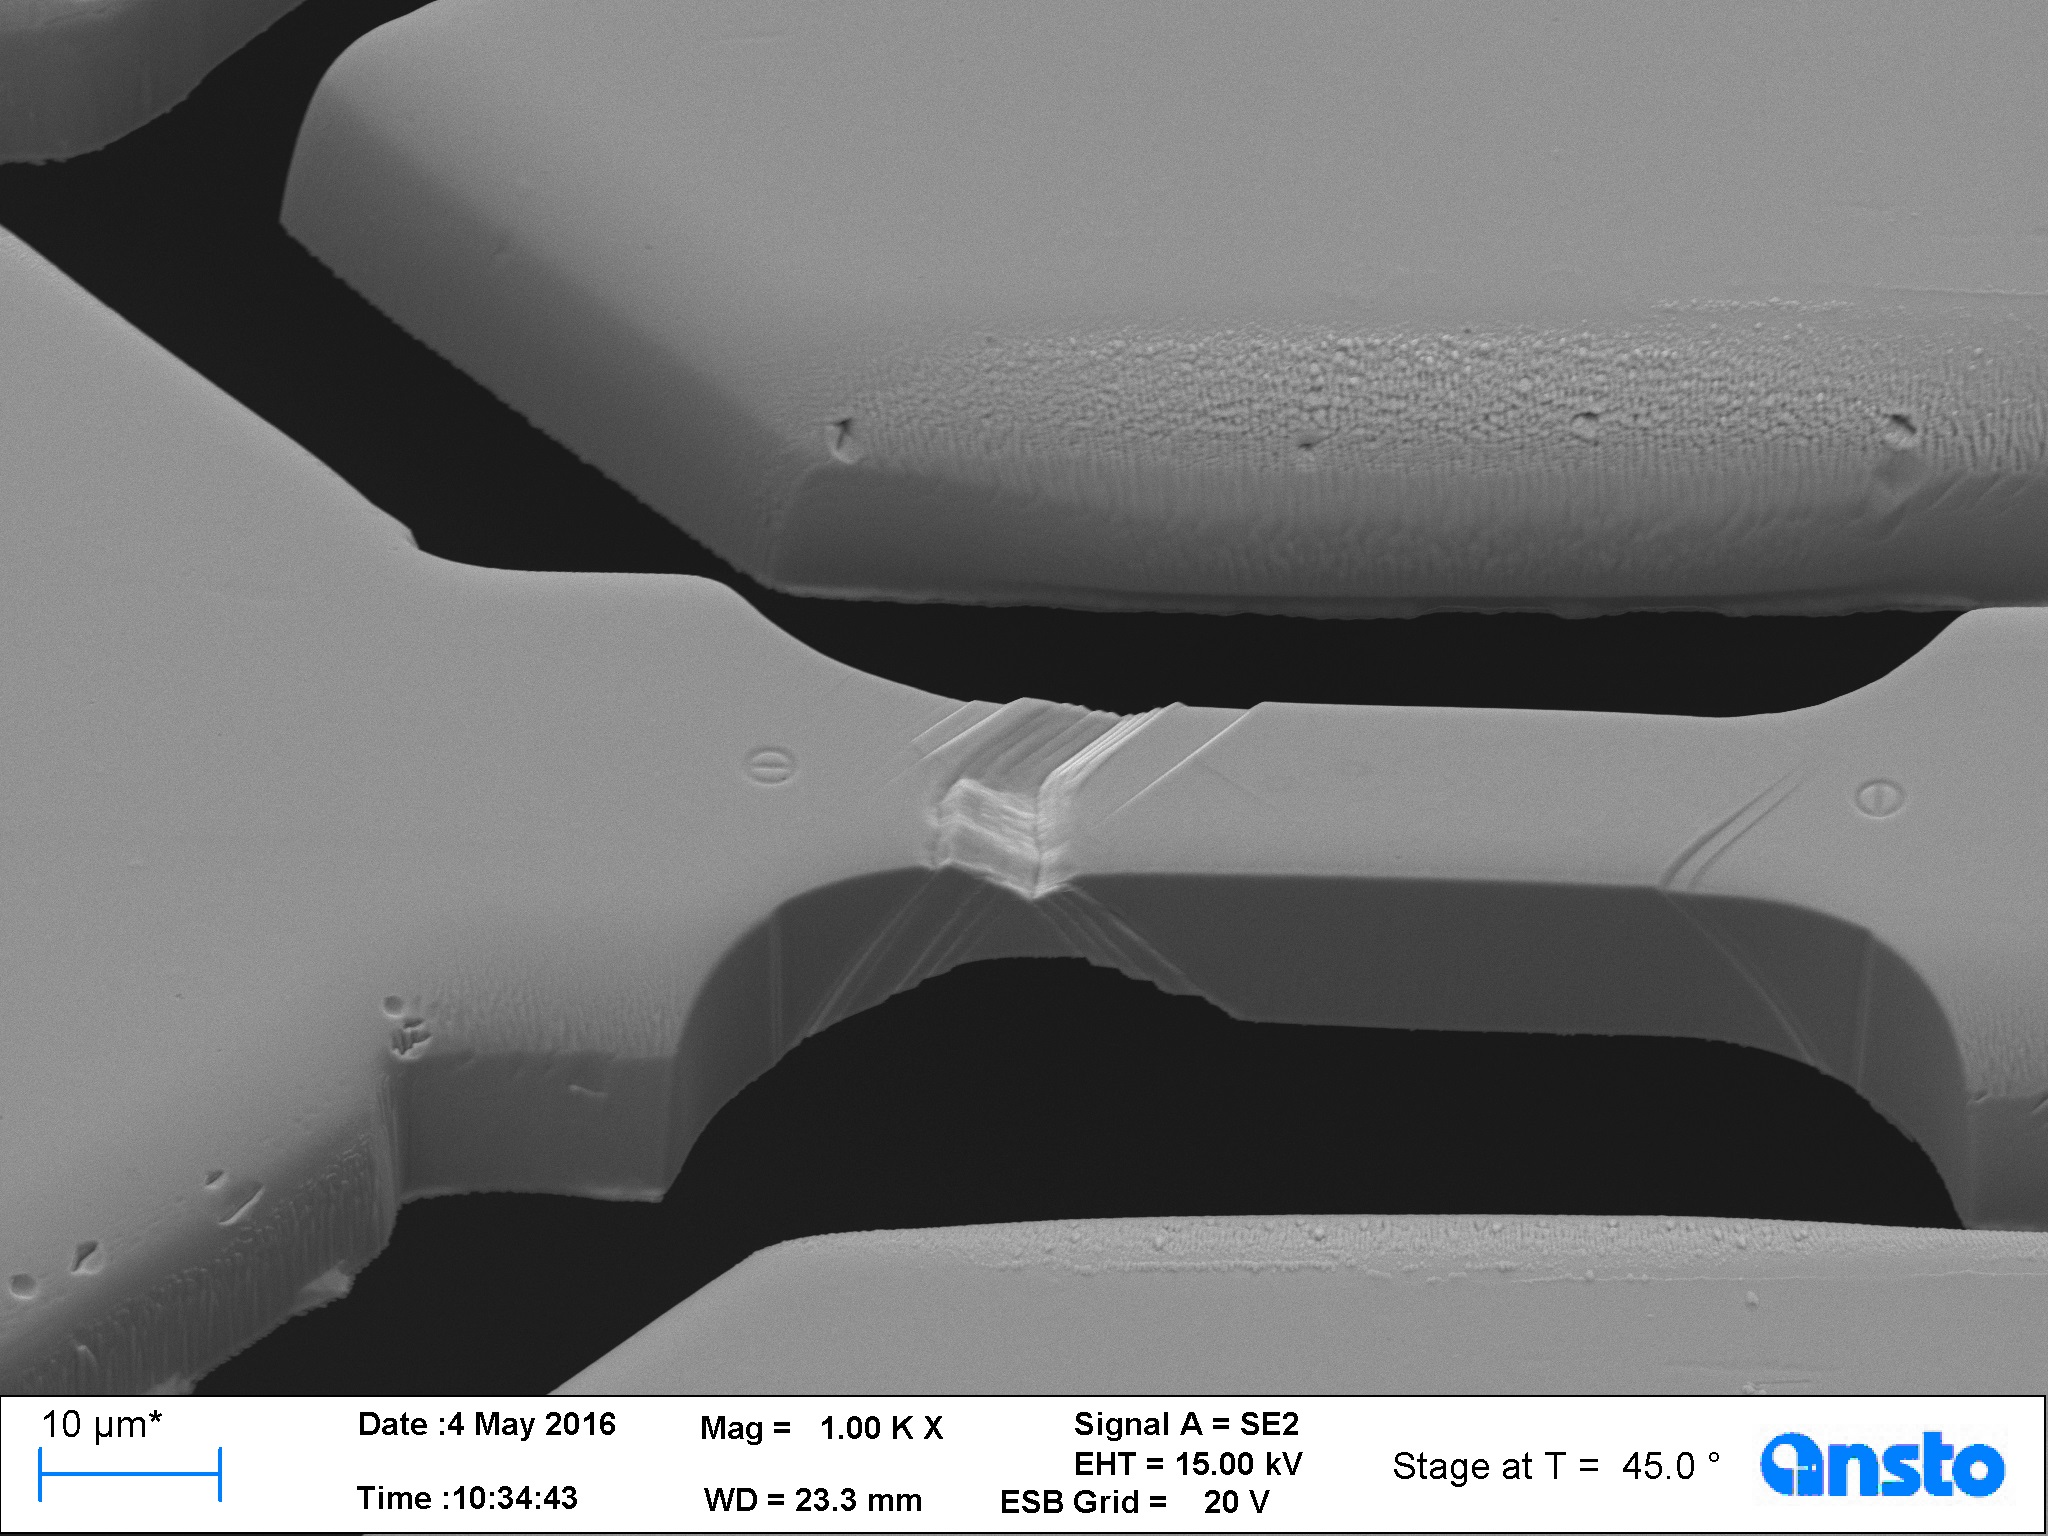
\includegraphics[width=\linewidth]{../data/Ni023.jpg}
    \end{subfigure}
    ~
    \begin{subfigure}[t]{0.3\linewidth}
        \centering
        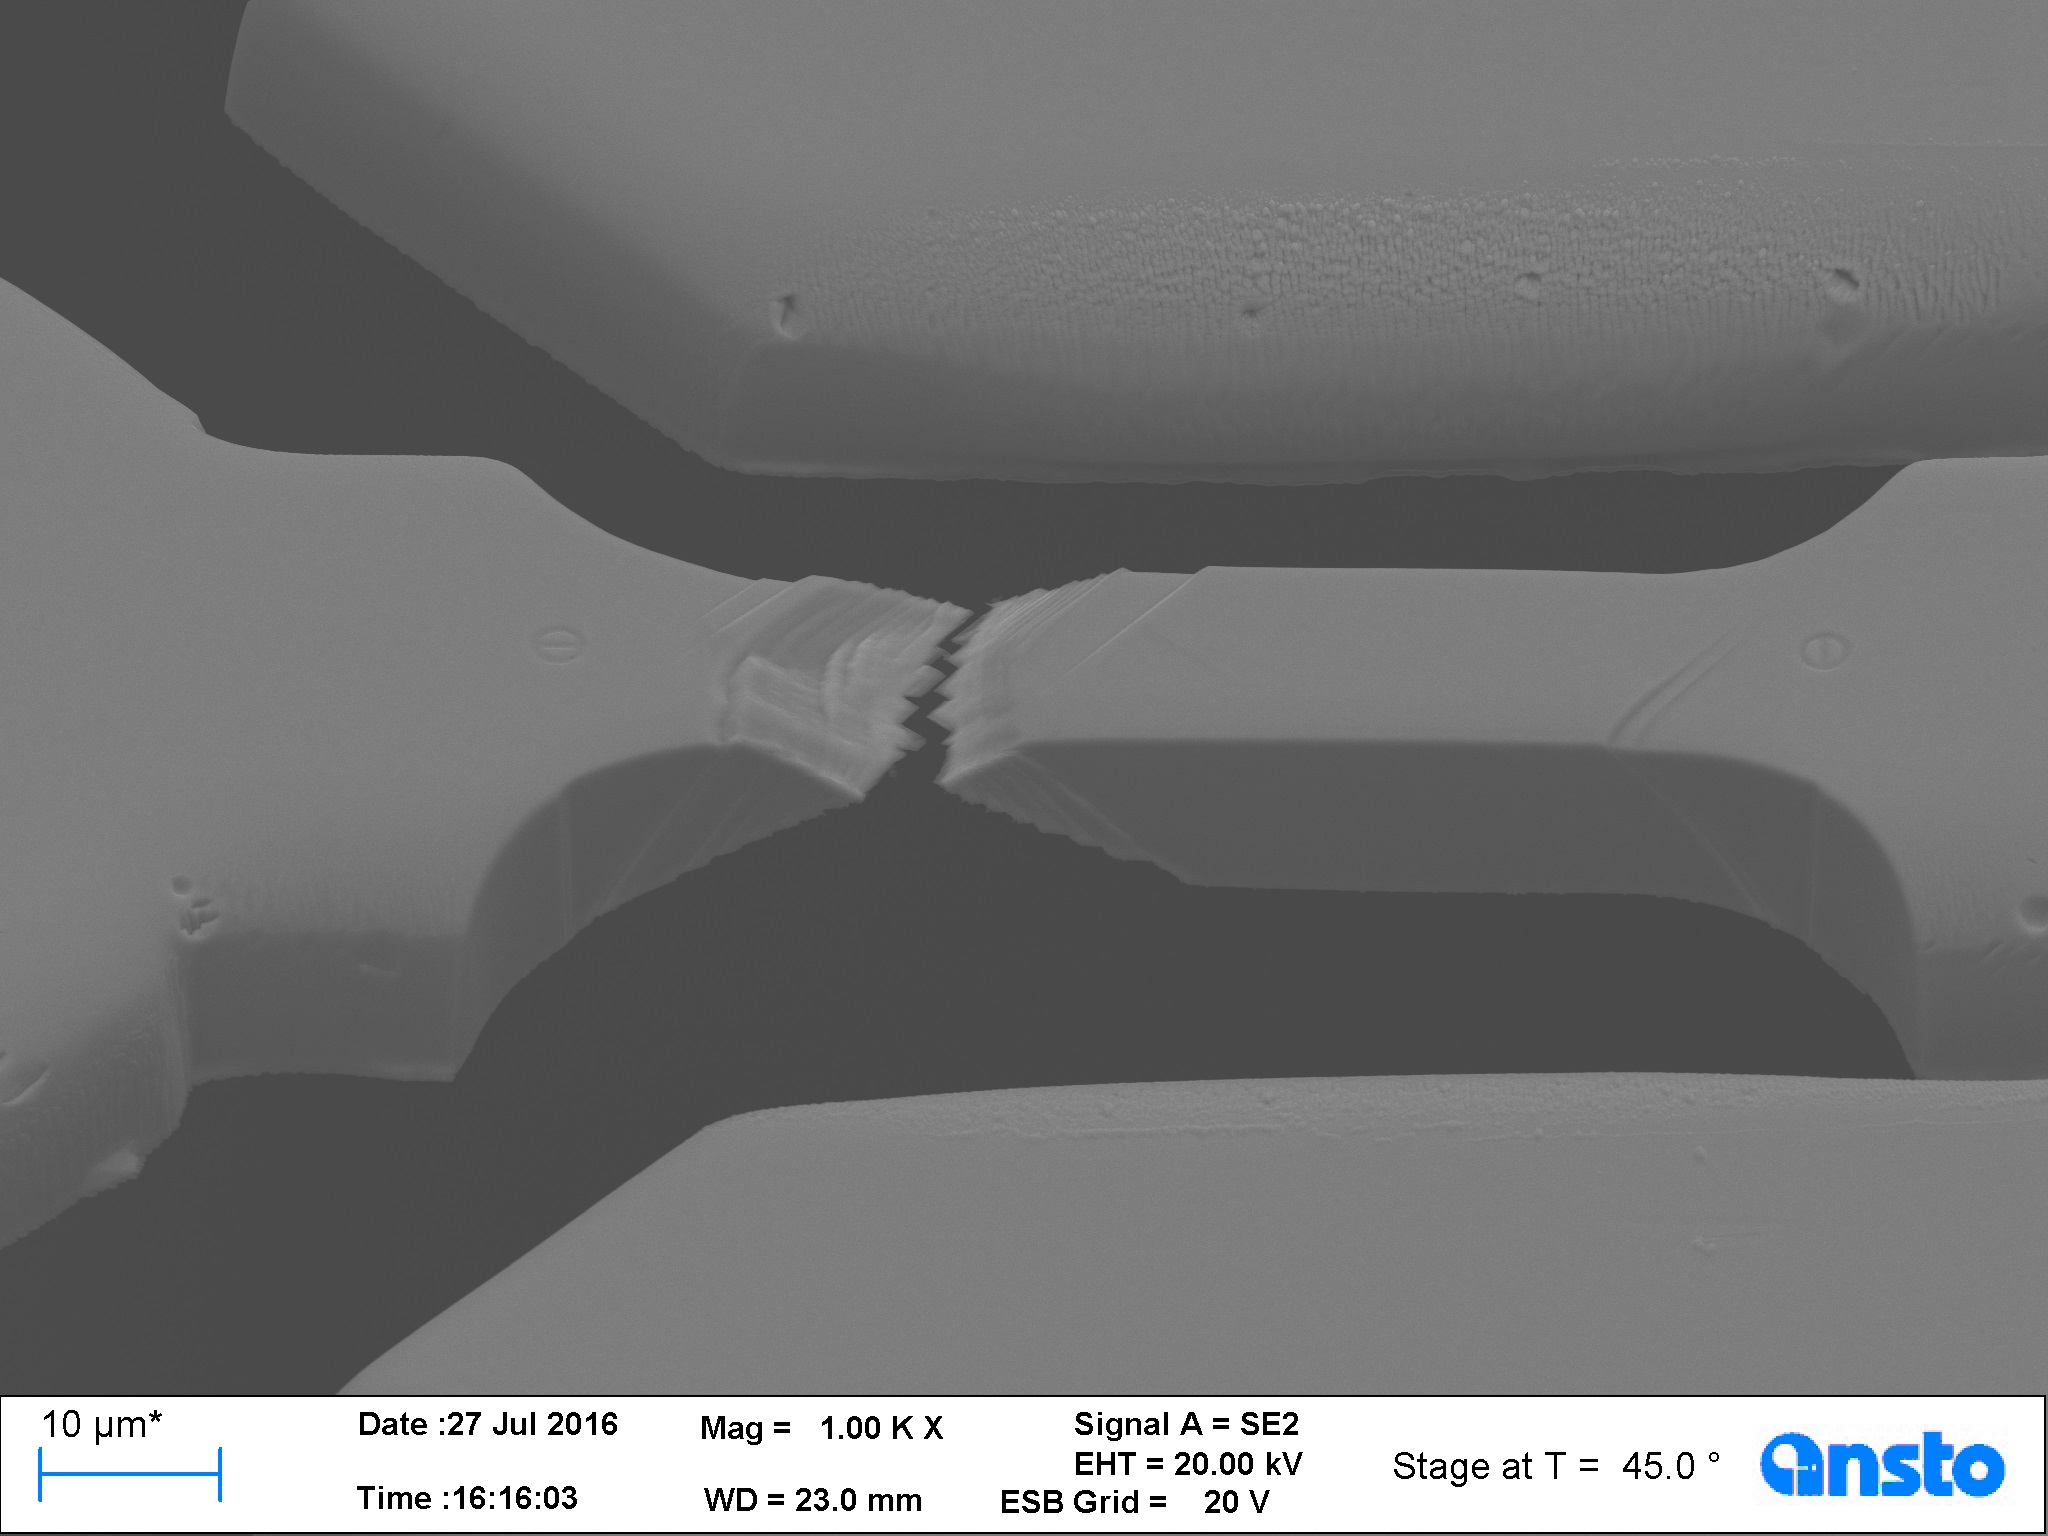
\includegraphics[width=\linewidth]{../data/Ni039.jpg}
    \end{subfigure}
    \caption{Tensile tests taken to failure.}
    \label{f:necking}
\end{figure}

It is worth noting that the timescale of dislocation plasticity simulations make them unsuitable to simulate the entirety of the experiments. EasyDD also does not have the capability to dynamically remesh its finite elements, so it cannot account for fracture.

\subsection{Dislocation plasticity setup}\label{s:nickelTensile}

We used prismatic loops with four sides as our Frank-Reed sources. Preliminary simulations showed the assumed dislocation density was too high, instead it was dropped to a single seed loop per active slip system. For the $\langle 1\, 0\, 0 \rangle$ loading direction this was 8 loops, and for $\langle 1\, 1\, 0 \rangle$ it was only 4; \cref{t:slipSystems} contains the active slip systems for both scenarios.
\begin{table}
    \centering
    \caption{Active slip systems for prismatic loops in the $\langle 1\, 0\, 0 \rangle$ and $\langle 1\, 1\, 0 \rangle$ tensile loading directions.}
    \label{t:slipSystems}
    \begin{tabular}{rcl}
        \toprule
        Loading direction                            & Slip plane    & Burgers vector           \\
        \midrule
        \multirow{8}{*}{$\langle 1\, 0\, 0 \rangle$} & $(1\, 1\, 1)$ & $[1\, \overline{1}\, 0]$ \\
                                                     & $(1\, 1\, 1)$ & $[1\, \overline{1}\, 0]$ \\
                                                     & $(1\, 1\, 1)$ & $[1\, \overline{1}\, 0]$ \\
                                                     & $(1\, 1\, 1)$ & $[1\, \overline{1}\, 0]$ \\
                                                     & $(1\, 1\, 1)$ & $[1\, \overline{1}\, 0]$ \\
                                                     & $(1\, 1\, 1)$ & $[1\, 0\, \overline{1}]$ \\
                                                     & $(1\, 1\, 1)$ & $[1\, 0\, \overline{1}]$ \\
                                                     & $(1\, 1\, 1)$ & $[1\, 0\, \overline{1}]$ \\
        \midrule
        \multirow{4}{*}{$\langle 1\, 1\, 0 \rangle$} & $(1\, 1\, 1)$ & $[1\, \overline{1}\, 0]$ \\
                                                     & $(1\, 1\, 1)$ & $[1\, \overline{1}\, 0]$ \\
                                                     & $(1\, 1\, 1)$ & $[1\, \overline{1}\, 0]$ \\
                                                     & $(1\, 1\, 1)$ & $[1\, 0\, \overline{1}]$ \\
        \bottomrule
    \end{tabular}
\end{table}

For the simulations, the pillar length was taken as $\SI{36}{\micro\metre}$, or $3\times$ the length of one of the sides of the square cross-section. The reason for this is to simulate dislocations moving into the bulk where they pile up, in the simulation, they stick to the end of the cantilever as per \cref{c:surfRem}.

We define surface node sets $\left\{\forall (x, y, z) \in [0,\, 1] \vert S_{xyz} \in \partial \hat{V}\right\}$, where $\hat{V}$ is a unit volume such that $S_{000}$ denotes the node at the origin, $S_{x00}$ the $x$-axis spanning edge at $y,\, z=0$, and $S_{xy0}$ the $xy$-plane at $z=0$. We use these node sets to define our neuman (displacement) boundary conditions as follows.
\begin{subequations}
    \begin{align}
        S_{0yz},\, S_{0y0},\, S_{0y1},\, S_{00z},\, S_{01z},\, S_{000},\, S_{001},\, S_{010},\, S_{011} & \gets u_x = 0        \\
        S_{01z},\, S_{010},\, S_{011}                                                                   & \gets u_y = 0        \\
        S_{0y0},\, S_{010},\, S_{000}                                                                   & \gets u_z = 0        \\
        S_{1yz},\, S_{1y0},\, S_{1y1},\, S_{10z},\, S_{11z},\, S_{100},\, S_{101},\, S_{110},\, S_{111} & \gets u_x = U > 0\,.
    \end{align}
\end{subequations}
In simple terms, the whole $yz$-plane at $x=0$ (including corner and edge nodes) is fixed at zero displacement in the $x$-direction; the whole $y$-edge at $x,\,z=0$ (including corner nodes) is also fixed at zero displacement in the $z$-direction; the whole $z$-edge at $x = 0\,\, y = 1$ (including corner nodes) is fixed at zero displacement in the $y$-direction; and the whole $yz$-plane (including corner and edge nodes) nodes at $x=1$ have a displacement, $U > 0$, applied in the $x$-direction ($U < 0$ would be a compressive load). All other degrees of freedom are free to move as necessary.

Once mapped to our simulated cuboid geometry, it looks like \cref{f:tensileSetup}.
\begin{figure}
    \centering
    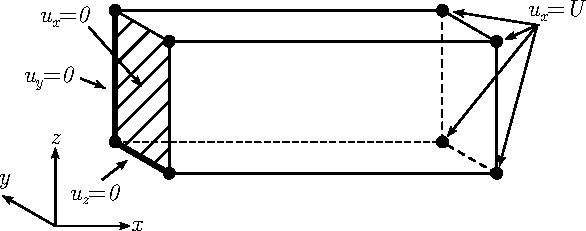
\includegraphics[width=0.8\linewidth]{tensileSetup.pdf}
    \caption[Displacement boundary conditions for dislocation plasticity modelling of single crystal, micro-tensile tests.]{Displacement boundary conditions for dislocation plasticity modelling of single crystal, micro-tensile tests.}
    \label{f:tensileSetup}
\end{figure}

In EasyDD, time is defined in units of shear modulus \cref{eq:timeConversion},
\begin{align}\label{eq:timeConversion}
    t_{\rvar{real}} & = t_{\rvar{sim}} \dfrac{B}{\lVert\mu\rVert}\,,
\end{align}
where $B \coloneqq 1 \times 10^{-4}[\si{\pascal}][\si{\second}]$ is the dislocation mobility and $\lVert\mu\rVert \coloneqq [\si{\pascal}]$ is the magnitude of the shear modulus (the shear modulus we use for the simulations is normalised to 1, its magnitude is used to scale parameters). The dislocation mobilities are normalised such that edge dislocations have mobility 1, other mobilities are defined from these. So the time conversion to real time is a matter of dividing the simulation time by the shear modulus.

The experimental loading rate provided was \SI{5}{\nano\metre/\second}, which when converted to simulation time, gives a loading rate that is far too low for the timescales we can model. So we defined $\Delta t_0 \equiv 5\times 10^{-9} \lVert\mu\rVert$ and found the maximum loading rate of the form $\dot{u} \equiv a \dfrac{\Delta l}{\Delta t_0}$, for which the quasi-static condition held true, where $\Delta l$ is the length of the beam in the loading direction and $a$ is a constant.

% size effects, microns

% 1
% 2
% 4
% 6
% 8
% 10

% dislocation density effects

% Current best loading rate for size effect
% % timeUnit = mumag * 1e6;
% % u\_dot = 1000*dx / timeUnit;

% timeUnit = 5e-3 * mumag * 1e6;
% u\_dot = 10*dx / timeUnit;

% try to push it as high as it can go without going wonky.
\subsection{Results and discussion}

\begin{figure}
    \centering
    \begin{subfigure}[t]{0.45\linewidth}
        \centering
        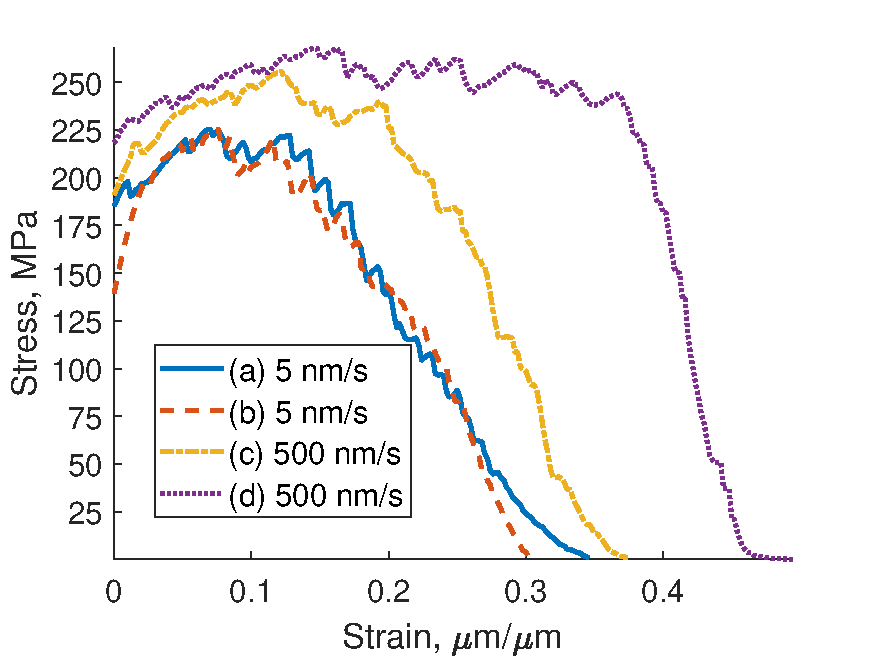
\includegraphics[width=\linewidth]{../data/Ni100.pdf}
        \caption[Tensile loading of Ni in the $\langle 1\, 0\, 0 \rangle$ direction.]{Tensile loading of Ni in the $\langle 1\, 0\, 0 \rangle$ direction.}
        \label{sc:Ni100}
    \end{subfigure}
    ~
    \begin{subfigure}[t]{0.45\linewidth}
        \centering
        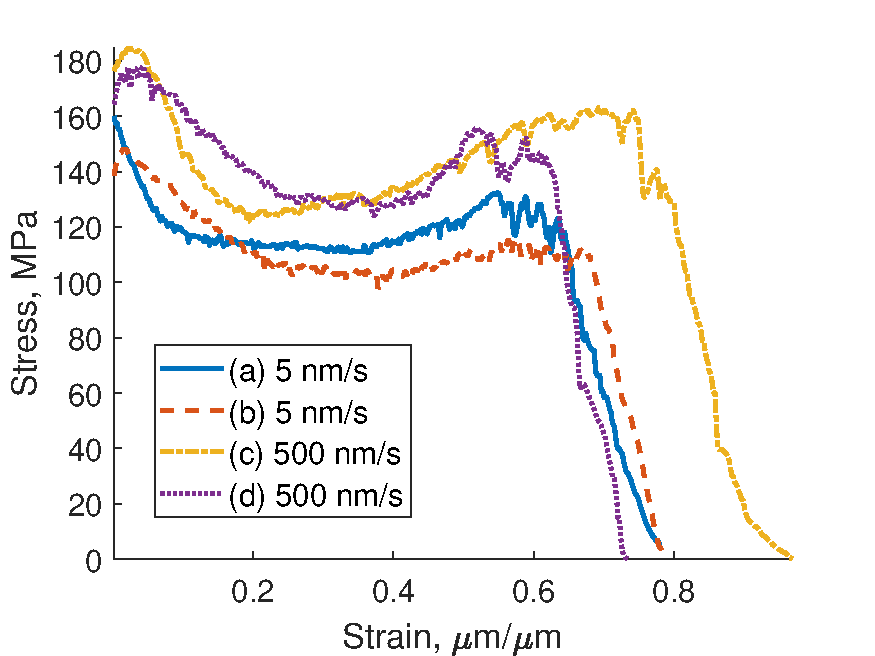
\includegraphics[width=\linewidth]{../data/Ni110.pdf}
        \caption[Tensile loading of Ni in the $\langle 1\, 1\, 0 \rangle$ direction.]{Tensile loading of Ni in the $\langle 1\, 1\, 0 \rangle$ direction.}
        \label{sc:Ni110}
    \end{subfigure}

    \begin{subfigure}[t]{0.45\linewidth}
        \centering
        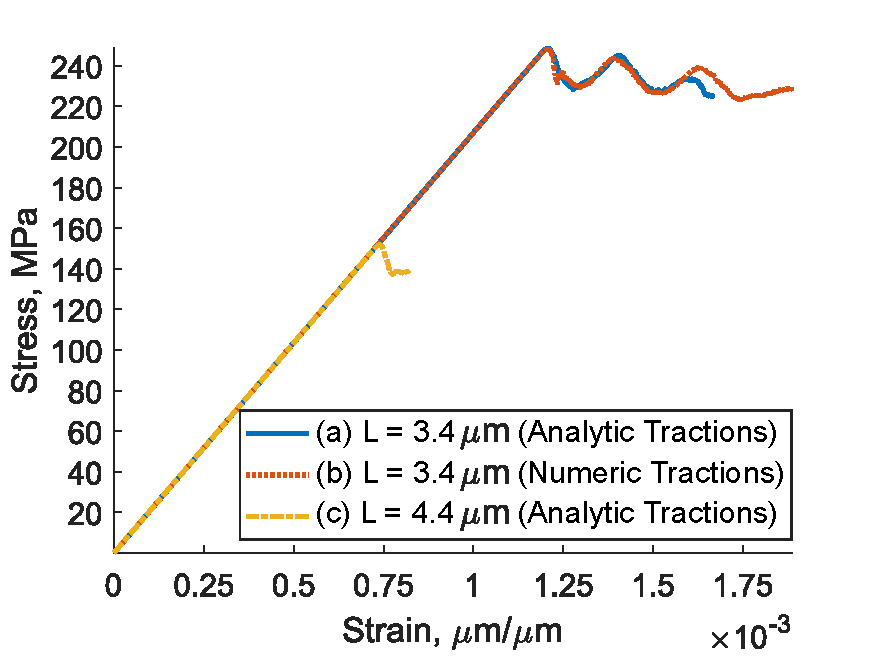
\includegraphics[width=\linewidth]{../data/Ni100_DDD.pdf}
        \caption[Dislocation-Plasticity simulation of tensile loading of Ni in the $\langle 1\, 0\, 0 \rangle$ direction.]{Dislocation-Plasticity simulation of tensile loading of Ni in the $\langle 1\, 0\, 0 \rangle$ direction.}
        \label{sc:Ni100_DDD}
    \end{subfigure}
    ~
    \begin{subfigure}[t]{0.45\linewidth}
        \centering
        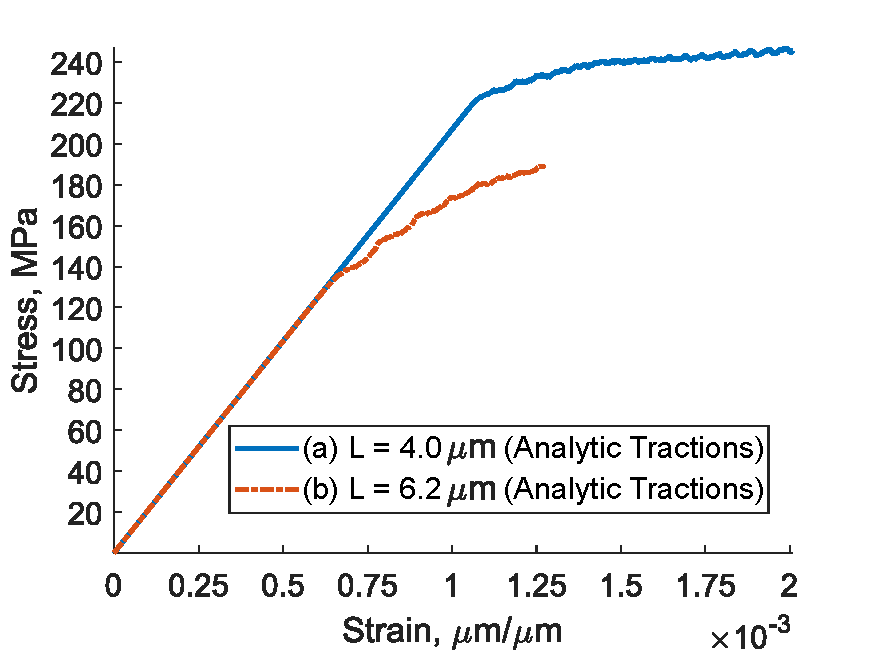
\includegraphics[width=\linewidth]{../data/Ni110_DDD.pdf}
        \caption[Dislocation-Plasticity simulation of tensile loading of Ni in the $\langle 1\, 1\, 0 \rangle$ direction.]{Dislocation-Plasticity simulation of tensile loading of Ni  in the $\langle 1\, 1\, 0 \rangle$ direction.}
        \label{sc:Ni110_DDD}
    \end{subfigure}
\end{figure}

\subsection{Conclusions}

\section{Tungsten cyclic loading and unloading cantilever}\label{s:tungstenCyclic}
\subsection{Introduction}
\subsection{Methodology}
\subsection{Results and discussion}
\subsection{Conclusions}

% 310


% TODO